\chapter{Methodology}\label{methodology}

This chapter outlines the research design, data collection methods, and analytical techniques employed in this study. The methodology is designed to ensure that the research objectives are met and that the findings are reliable and valid.


\section{Dataset Acquisition}

In this section explain how dataset used in the study has been acquired. If you have acquired the dataset from any repository link to that repository must be added and also provided in the citation section. Provide \href{https://example.com/record/2000}{\textcolor{blue}{hyperlink}} if necessary. 

Also, provide a slight description of the dataset and mention any data collection that is ongoing and what specific method you are using to collect the data.


\section{Dataset Details}

Provide details about your dataset. You can also provide a snapshot of sample data here to better explain your dataset.

Split your explanation into multiple subsection if necessary.


\subsection{Data Type 1}

Explanation of data type 1. Provide figure if necessary

\begin{figure}[htb ]
    \centering
    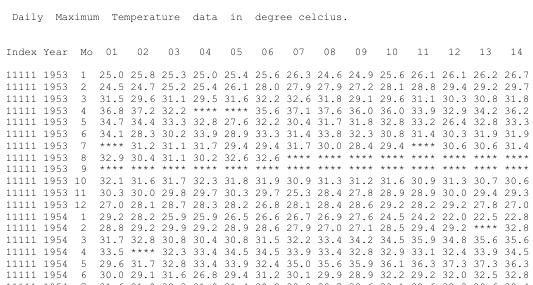
\includegraphics[width=.75\textwidth]{figures/demoFigure2.png}
    \caption{Demo Data Screenshot}
    \label{fig:dataDemo}
\end{figure}

\subsection{Data Type 2}
Explanation of data type 2. Provide tables and figures if necessary

You can write table here like this \ref{tab:numerical_data}.
\begin{table}[h]
    \centering
    \caption{Summary of Numerical Data}
    \label{tab:numerical_data} 
    \begin{tabular}{|c|c|c|c|}
        \hline
        \textbf{ID} & \textbf{Value 1} & \textbf{Value 2} & \textbf{Total} \\ 
        \hline
        1 & 10 & 15 & 25 \\ 
        2 & 20 & 25 & 45 \\ 
        3 & 30 & 35 & 65 \\ 
        4 & 40 & 45 & 85 \\ 
        \hline
    \end{tabular}
\end{table}

You can also include table from external file like \ref{tab:sampleTable}
% Include the table from the external file
\begin{table}[ht]
    \centering
    \caption{Sample Table}
    \label{tab:sampleTable}
    \begin{tabular}{|c|c|c|}
        \hline
        Column 1 & Column 2 & Column 3 \\
        \hline
        Data 1 & Data 2 & Data 3 \\
        Data 4 & Data 5 & Data 6 \\
        \hline
    \end{tabular}
\end{table}


\section{Data Preprocessing}

Explain all the preprossessing done to the dataset in this section. Explain each preprocessing step in individual subsections.

\subsection{Preprocessing 1}
Explain Preprocessing step 1.


\subsection{Preprocessing 2}
Explain Preprocessing step 2.



\section{Dataset insights}
Explain the insight found after the initial preprocessing of the dataset.
\subsection{Correlation Matrix}

\subsection{Insight 2}

\section{Primary training}
Explain how you initially trained your model including all the algorithms used. Provide details about each algorithms.



\section{Data Refinement}
Explain any refinements done in the dataset or preprocessing of dataset done to improve your outcome.


\subsection{Refinement 1}

\subsection{Refinement 2} 


\newpage


\section{Secondary/Final Training}
Explain your final training steps here.

\section{Final Model}
Explain your final model here. You should provide necessary figures to explain your model. All figures should be clear and readable. If necessary you can add figures from PDF files. 

\begin{figure}[h]
    \centering
    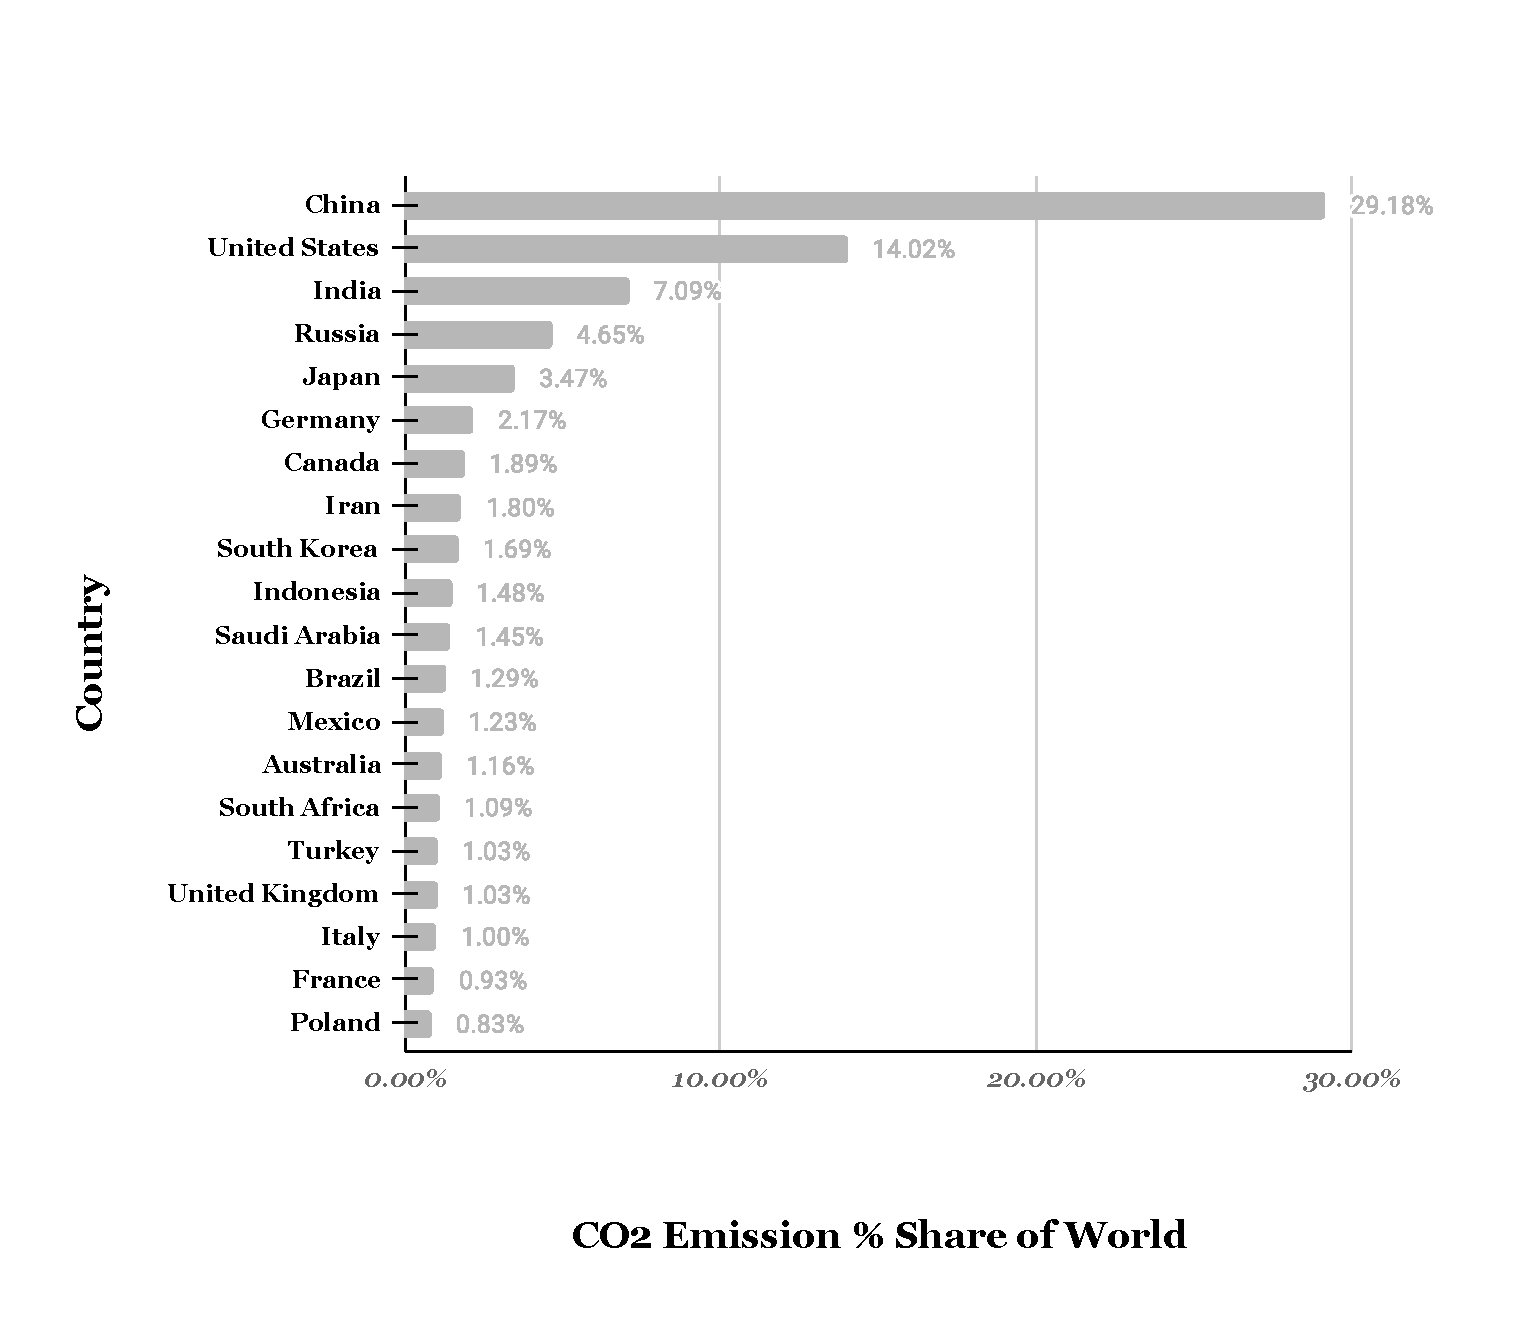
\includegraphics[width=.75\textwidth]{figures/demoFigure3.pdf}
    \caption{Demo Chart}
    \label{fig:dataChart}
\end{figure}



\section{Ethical Considerations}

Provide any ethical considerations you took for your studies and any approval from  Institutional Review Board (IRB).

\section{Limitations}

What are some limitations of your study? Explain it here.